\section{Introduction}

Smart homes are equipped with a myriad of sensor and actuator devices that can enable complex services to assist residents. Smart-home software, collectively called ``apps"~\cite{ALAA201748}, is now getting increasingly complex, thanks to increasing needs for customisation as well as the introduction of innovative and disruptive devices and IoT technologies.  Fig.~\ref{figure:SmartHome}  shows a typical smart home with sensors for light intensity, dust levels and motion, as well as actuators such as lighting, refrigerator, etc. These devices can be controlled by one or more apps to provide customised services and care for the residents. 

\begin{figure}[!h]
    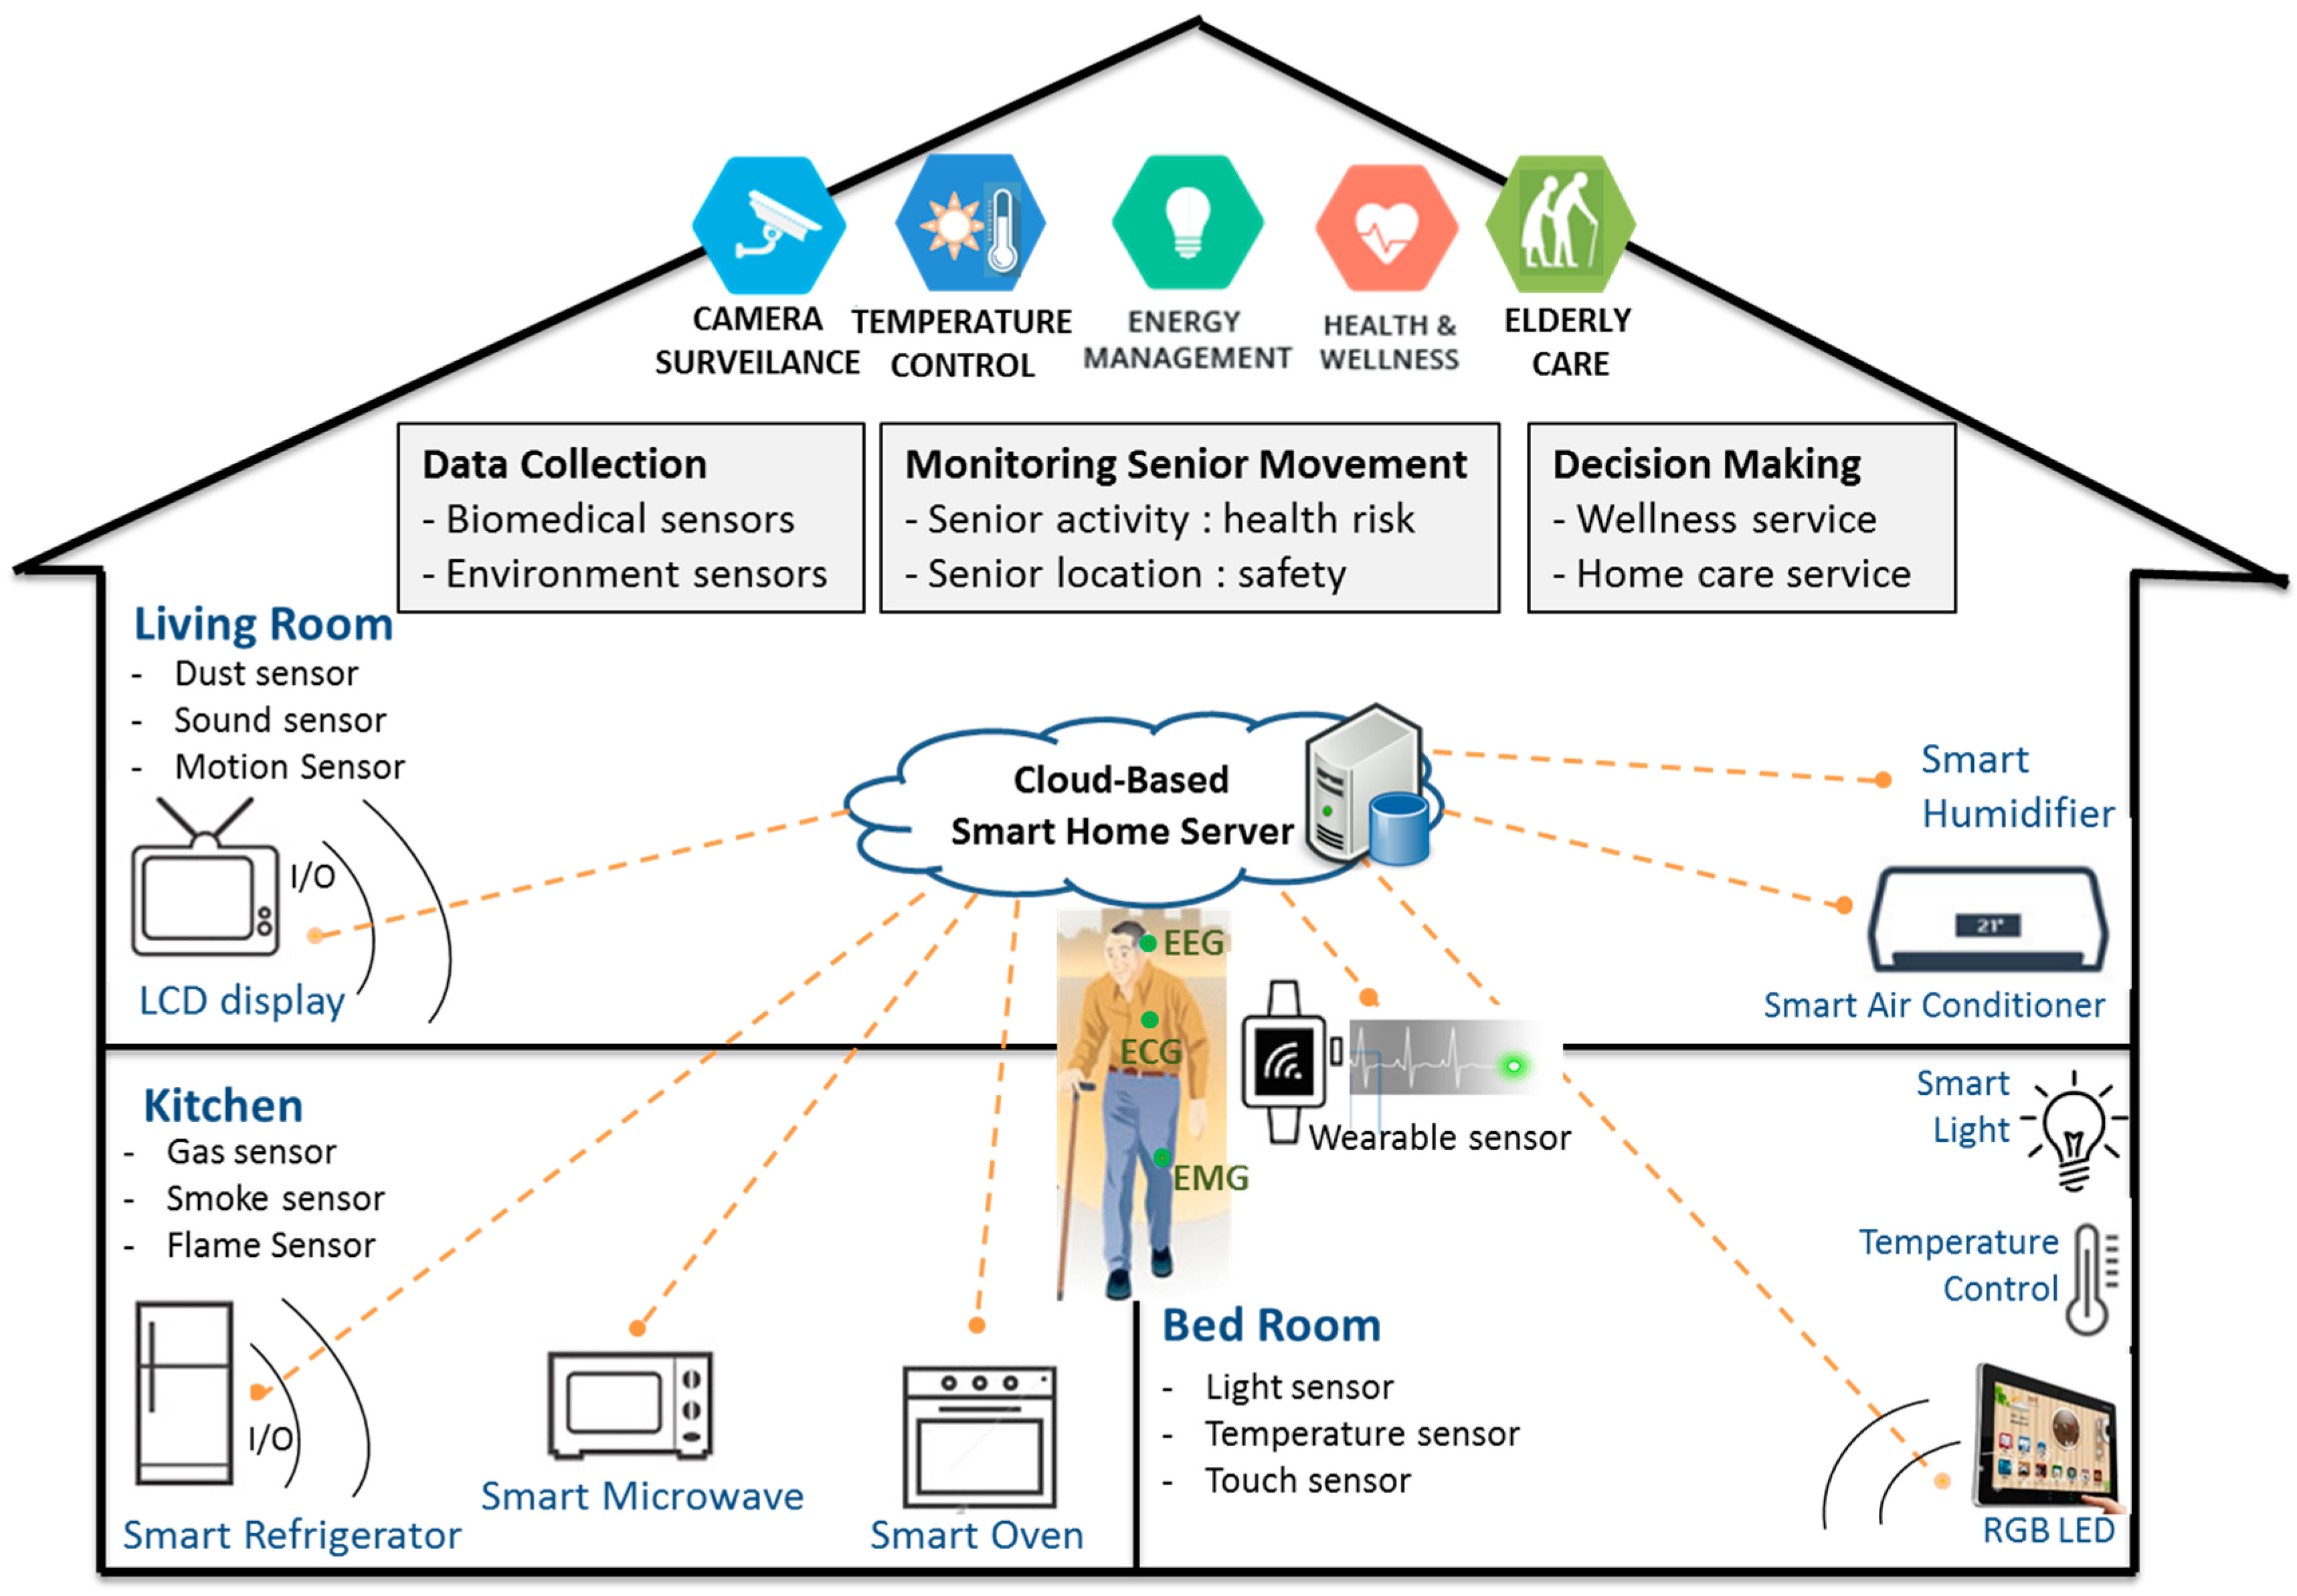
\includegraphics[width=\textwidth]{figs/smarthome}
    \caption{Smart Home \cite{jung2017hybrid}}
    \label{figure:SmartHome}
\end{figure}



There are a number of gaps in current research on designing smart home apps. 
These include a lack of interoperability between devices resulting in higher costs of deploying services~\cite{stojkoska2017review}, and implementing security measures such as confidentiality, integrity and availability~\cite{schneps2012wired}. Many current solutions target some of these problems, but often  fail to be effective in terms of usability which is a very important factor in the adoption of this technology. 

This paper focuses on the problem of easily creating and deploying smart-home apps. Existing tools or design models to create these apps cannot be readily used by non-experts, such as medical experts wanting to design apps for in-home care of their patients. Technically, the problem addressed in this paper is to efficiently and automatically generate correct code for these apps from \textit{behavioural} diagrams. Behavioral diagrams have been identified in this paper as more usable for non-experts wanting to design smart home apps (Sec.~\ref{sec:relatedworks}.
Also, existing automatic code-generators only work for \textit{structural} diagrams, such as UML Class Diagrams~\cite{rumpe2016modeling}.
This research addresses the following research questions:

\begin{enumerate}
\item \textbf{\textit{RQ1}} - Which factors lead to the choice of an app design model to address the challenges such as lack of interoperability between devices at the software level? 
\item \textbf{\textit{RQ2}} - What are the architectural characteristics of an automatic translation tool to convert an app design (based on the model developed after answering \textit{\textbf{RQ1}}) into a customized smart home app?
\item \textbf{\textit{RQ3}} - How can the high-level architecture of an automatic translation tool obtained from \textit{\textbf{RQ3}} lead towards the implementation of a prototype automatic translation tool?
\end{enumerate}




The design of this research followed a systematic literature review to refine and answer RQ1 and RQ2, and an adapted Design Science methodology to design and develop a solution to answer RQ3.
Fig.~\ref{figure:solution} shows an overview of the features of the solution, called the automatic translation tool. 
The tool automatically generates executable Java code from a UML Activity Diagram.
Activity Diagrams were identified as the most appropriate model for smart home apps while answering RQ1 (see Sec.~\ref{sec:relatedworks}).
The Eclipse-based automatic translation tool offers a fully featured editor for designing smart home apps.
The tool includes a compiler which accepts a visual plan, expressed as a UML activity diagram, and translates the visual plan into a runnable code which can then be deployed to a smart home application. 
An evaluation of the tool shows that the editor has high usability, and the compiler generates error-free and compact code, which can be deployed easily into any smart-home. 


%Pic1
\begin{figure}[!ht]
	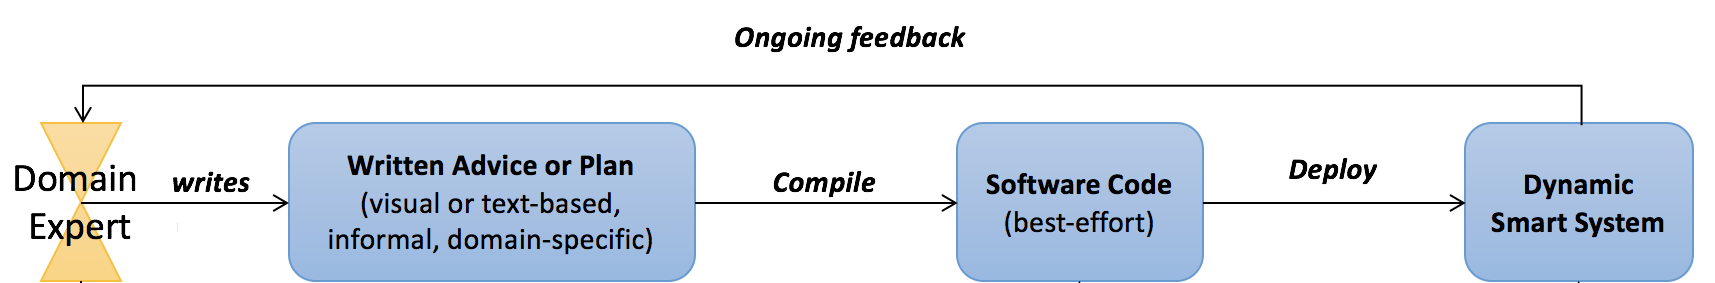
\includegraphics[width=\textwidth]{figs/Proposed_Solution}
	\caption{Overview of the automatic translation tool}
	\label{figure:solution}
\end{figure}


The primary contributions of this paper are:

\begin{enumerate}
\item \textbf{Choosing UML Activity Diagram as the more appropriate app design model for designing smart-home apps.} UML Activity diagrams are easier to use for non-experts due to their similarity with flowcharts, and also because they capture behavioral aspects rather than the structural aspects of a program. 

\item \textbf{User-friendly and fully-featured UML Activity Diagram Editor.} The editor features strong UML activity diagramming features, model element relationships and navigation among the model elements between the model editing space and the customized palette. Moreover, the editor can be used to design any smart home app. 

\item \textbf{Effective and Automatic Code Generation from Behavioral UML Activity Diagrams.} We have developed a compiler to generate correct executable Java code from UML activity diagrams that can be deployed in any smart home via a smart-phone.


\end{enumerate}






